\documentclass[a4paper,10pt]{article}

\usepackage[margin=2cm]{geometry}
\usepackage{graphicx}
\usepackage{amsmath}
\usepackage{array}
\usepackage{hyperref}
\usepackage[all]{hypcap}
\usepackage{listings}
\lstdefinestyle{TerminalStyle}{
  language=bash,
  basicstyle=\small\sffamily,
  numbers=left,
  numberstyle=\tiny,
  numbersep=3pt,
  frame=tb,
  columns=fullflexible,
  linewidth=0.9\linewidth,
  xleftmargin=0.1\linewidth
}
\lstdefinestyle{HtmlStyle}{
  language=html,
  basicstyle=\small\sffamily,
  numbers=left,
  numberstyle=\tiny,
  numbersep=3pt,
  frame=tb,
  columns=fullflexible,
  linewidth=0.9\linewidth,
  xleftmargin=0.1\linewidth
}
\lstdefinestyle{OutputStyle}{
  language=html,
  basicstyle=\small\sffamily,
  frame=tb,
  columns=fullflexible,
  linewidth=0.9\linewidth,
  xleftmargin=0.1\linewidth
}

\setlength{\parindent}{0pt}
\setlength{\parskip}{1ex plus 0.5ex minus 0.2ex}
\title{
\includegraphics[width=12cm]{Eeufeeslogo.jpg} \\
       Department of Computer Science \\
       University of Pretoria \\
       \vspace{0.5cm}
       Software Engineering\\
       COS301 Main Project \\
       \vspace{1.0cm}
       \begin{large} \textbf{Team CodeX}\\ ReRoute Purchasing Management Systems\end{large}\\
       \vspace{1.0cm}
       User Manual \\}
       
\date{August 10, 2017} 
\author{}

\begin{document}
\maketitle
\thispagestyle{empty}
\clearpage

\newpage
\pagenumbering{roman}
\thispagestyle{empty}
\tableofcontents
\clearpage

\newpage
\pagenumbering{arabic}

\section{Introduction}
Reroute Systems is a software company with different in-house developed applications. The Purchase Management System 
application specifically, is the main application and mainly active in the pharmaceutical space.\\
This document contains guidelines on how the application works, and how one can maximise the application and all it entails for best use.\\

\section{General Information}
\subsection{Title Page}
This application is the Reroute Purchasing Management System affiliated with the Reroute Systems company.\

For best use, it is advised that users have background knowledge in the pharmaceutical space.\\

\subsection{System Overview}
The system is a search engine called \textbf{Smart Search} which is enriched with functionality of performing advanced search in order to retrieve a product information in a master file given some values such as the product name, etc. The system aims to perform an AI search which will make it efficient and fast to retrieve the suitable product information. \\
	
	\subsubsection{Stakeholders}
	The stakeholders of the system include the following:
	\begin{itemize}
	\item \textbf{The Client} is Diederik Mostert, Software Director of ReRoute Systems who proposed the project as a result of a challenge faced in the company, which is to search a product on master file with different combination used by each wholesaler.
	\item \textbf{Users in Pharmaceutical space} They will use the system to retrieve information of the product they need.
	\end{itemize}
\subsection{System Configuration}

\subsection{Installation}
To be implemented.

\section{Getting started}
	The application design looks as follows: \\
	\subsection{Main screen}
	When the app is launched it requires your login credentials.\\
	{\centering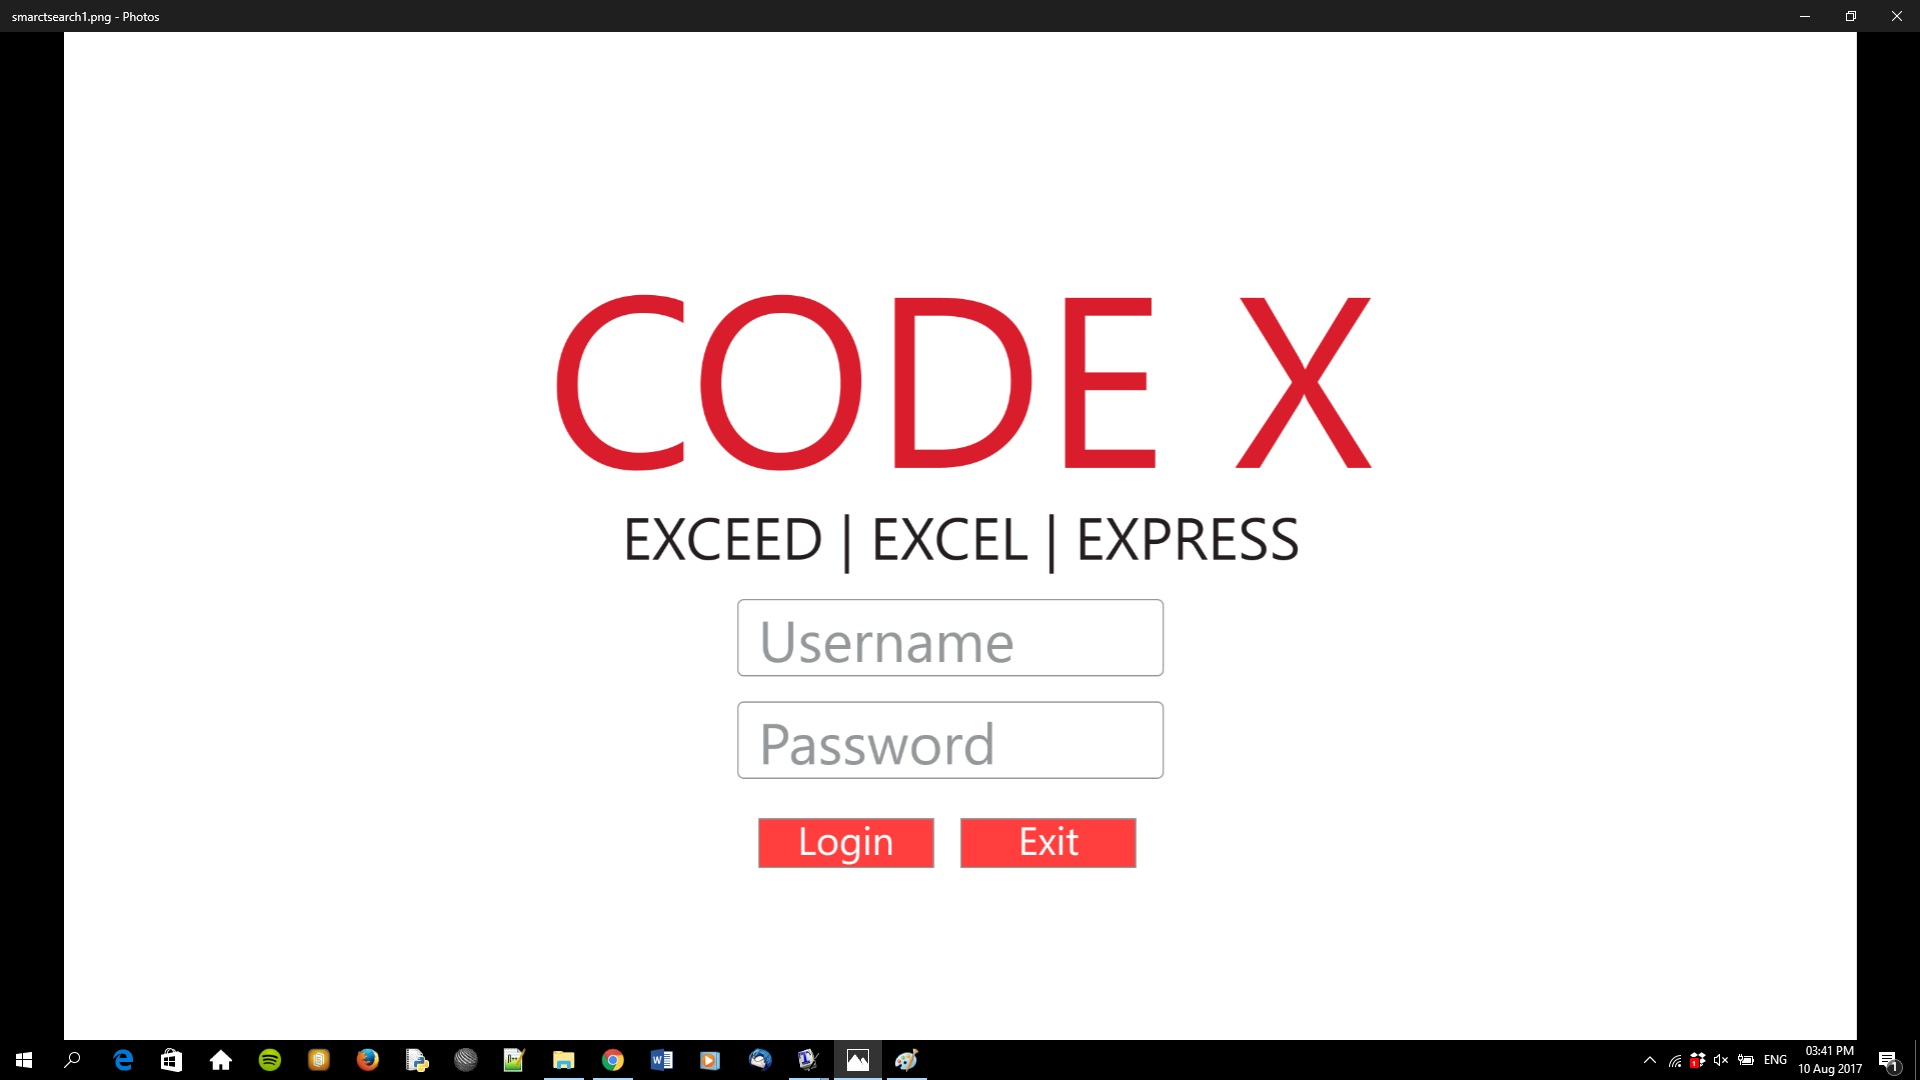
\includegraphics[width=15cm, scale=0.5]{smarctsearch1.jpg}}
	\subsection{Search Menu}
	The search screen where the user enter the product related information. \\
	{\centering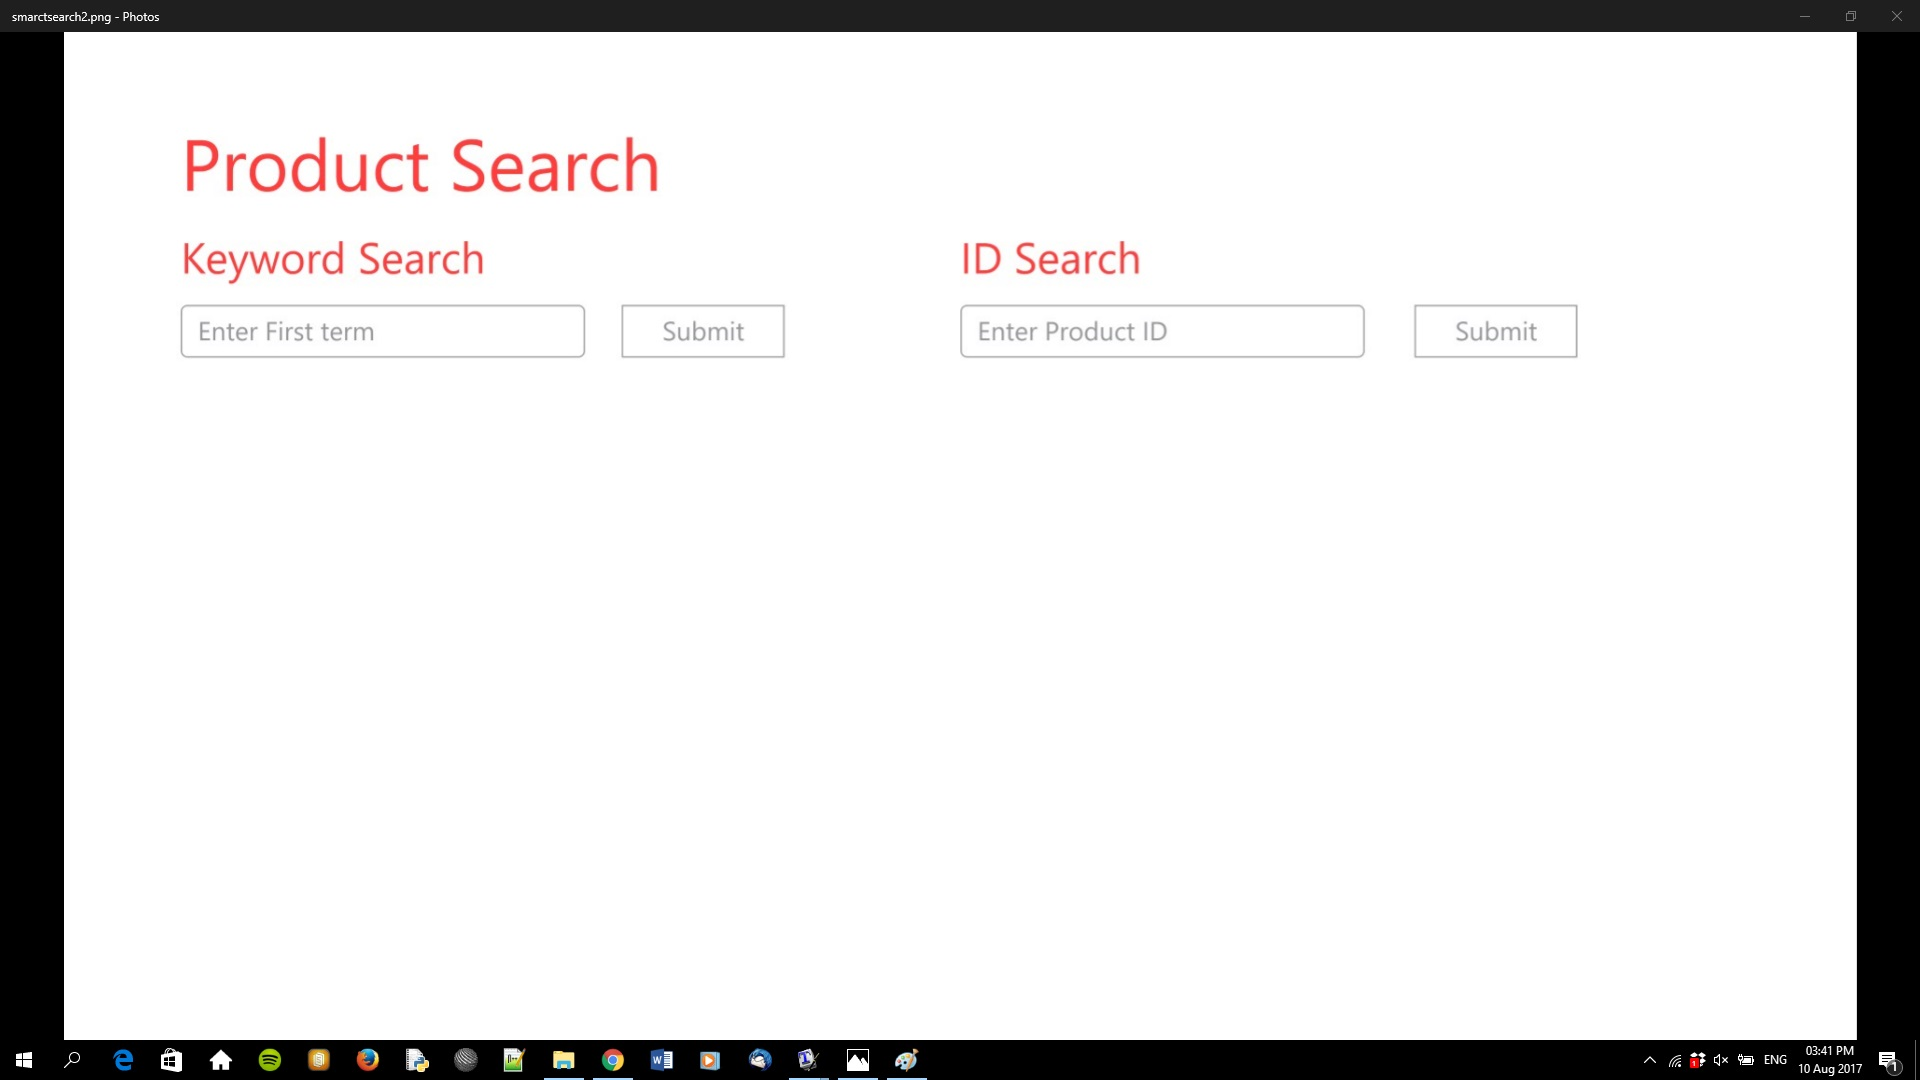
\includegraphics[width=15cm, scale=0.5]{smarctsearch2.jpg}} \\ \\
	{\centering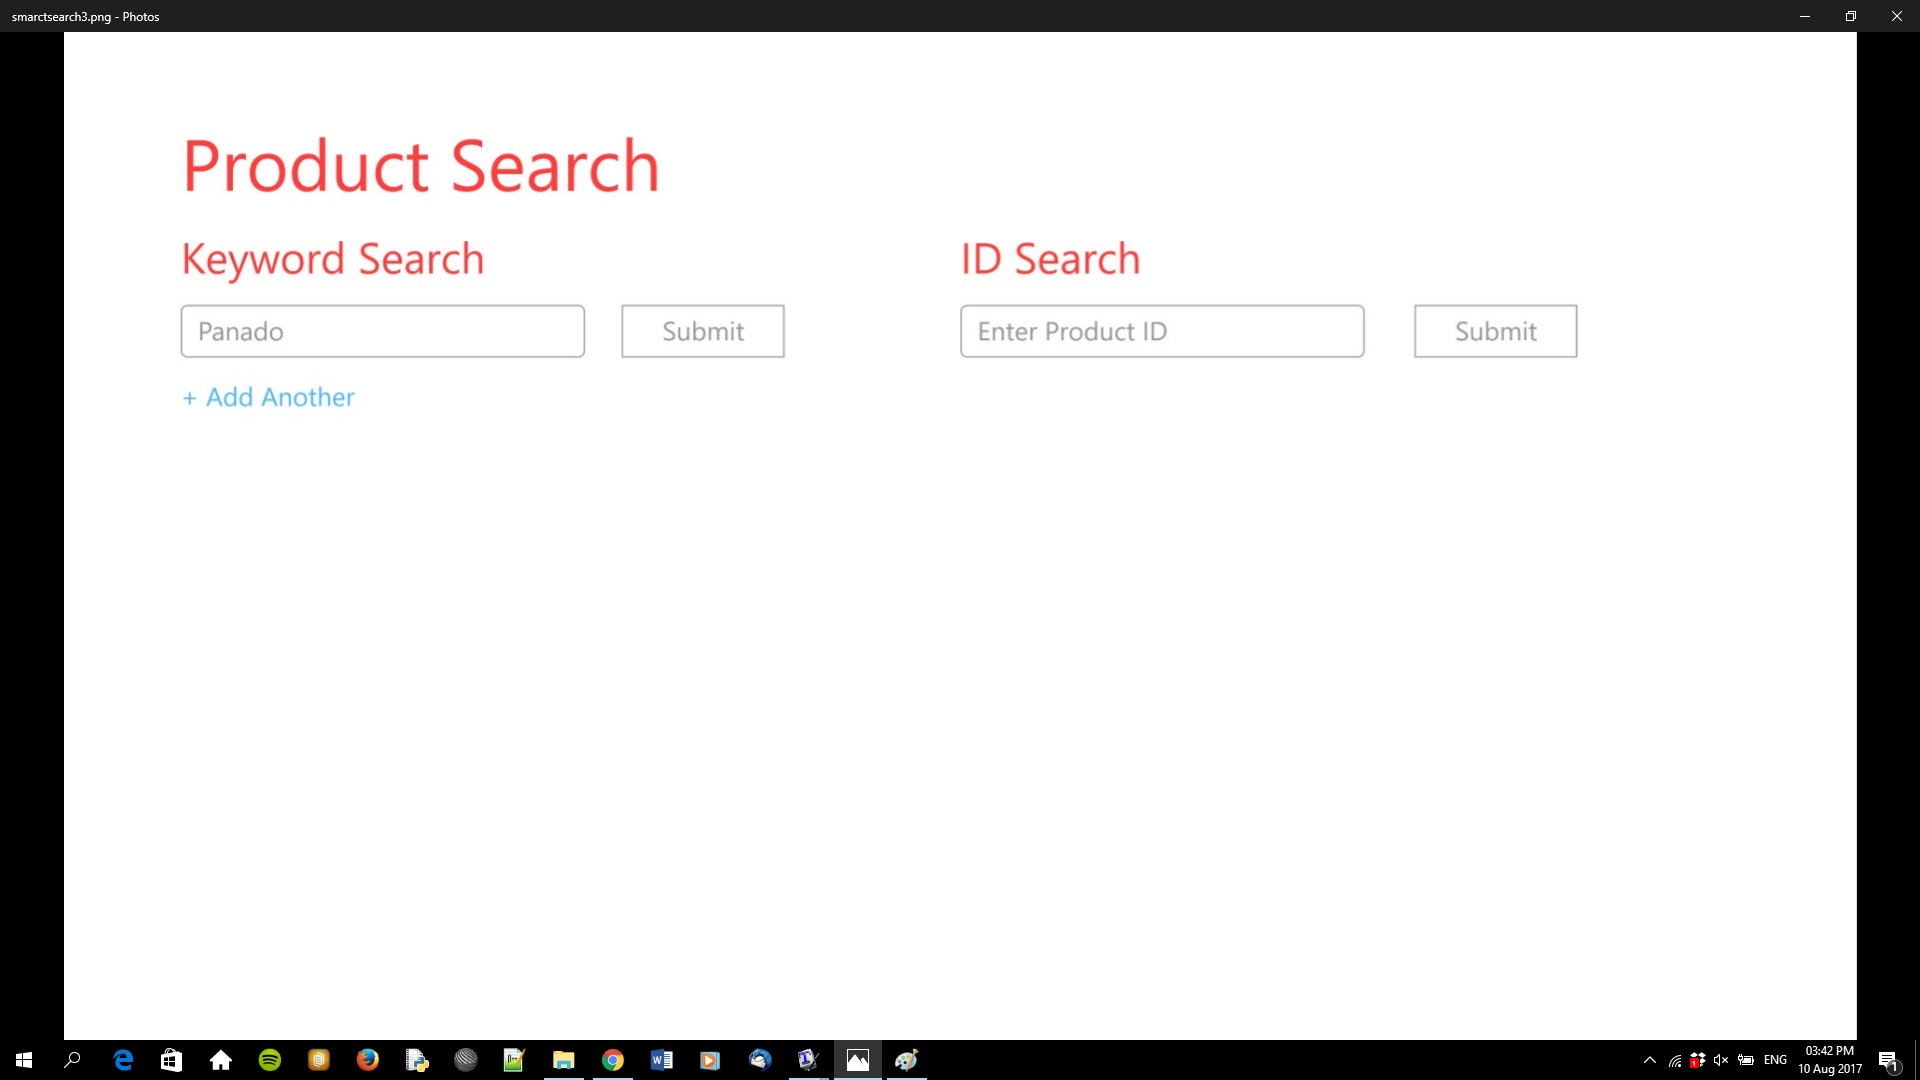
\includegraphics[width=15cm, scale=0.5]{smarctsearch3.jpg}} \\ \\
	{\centering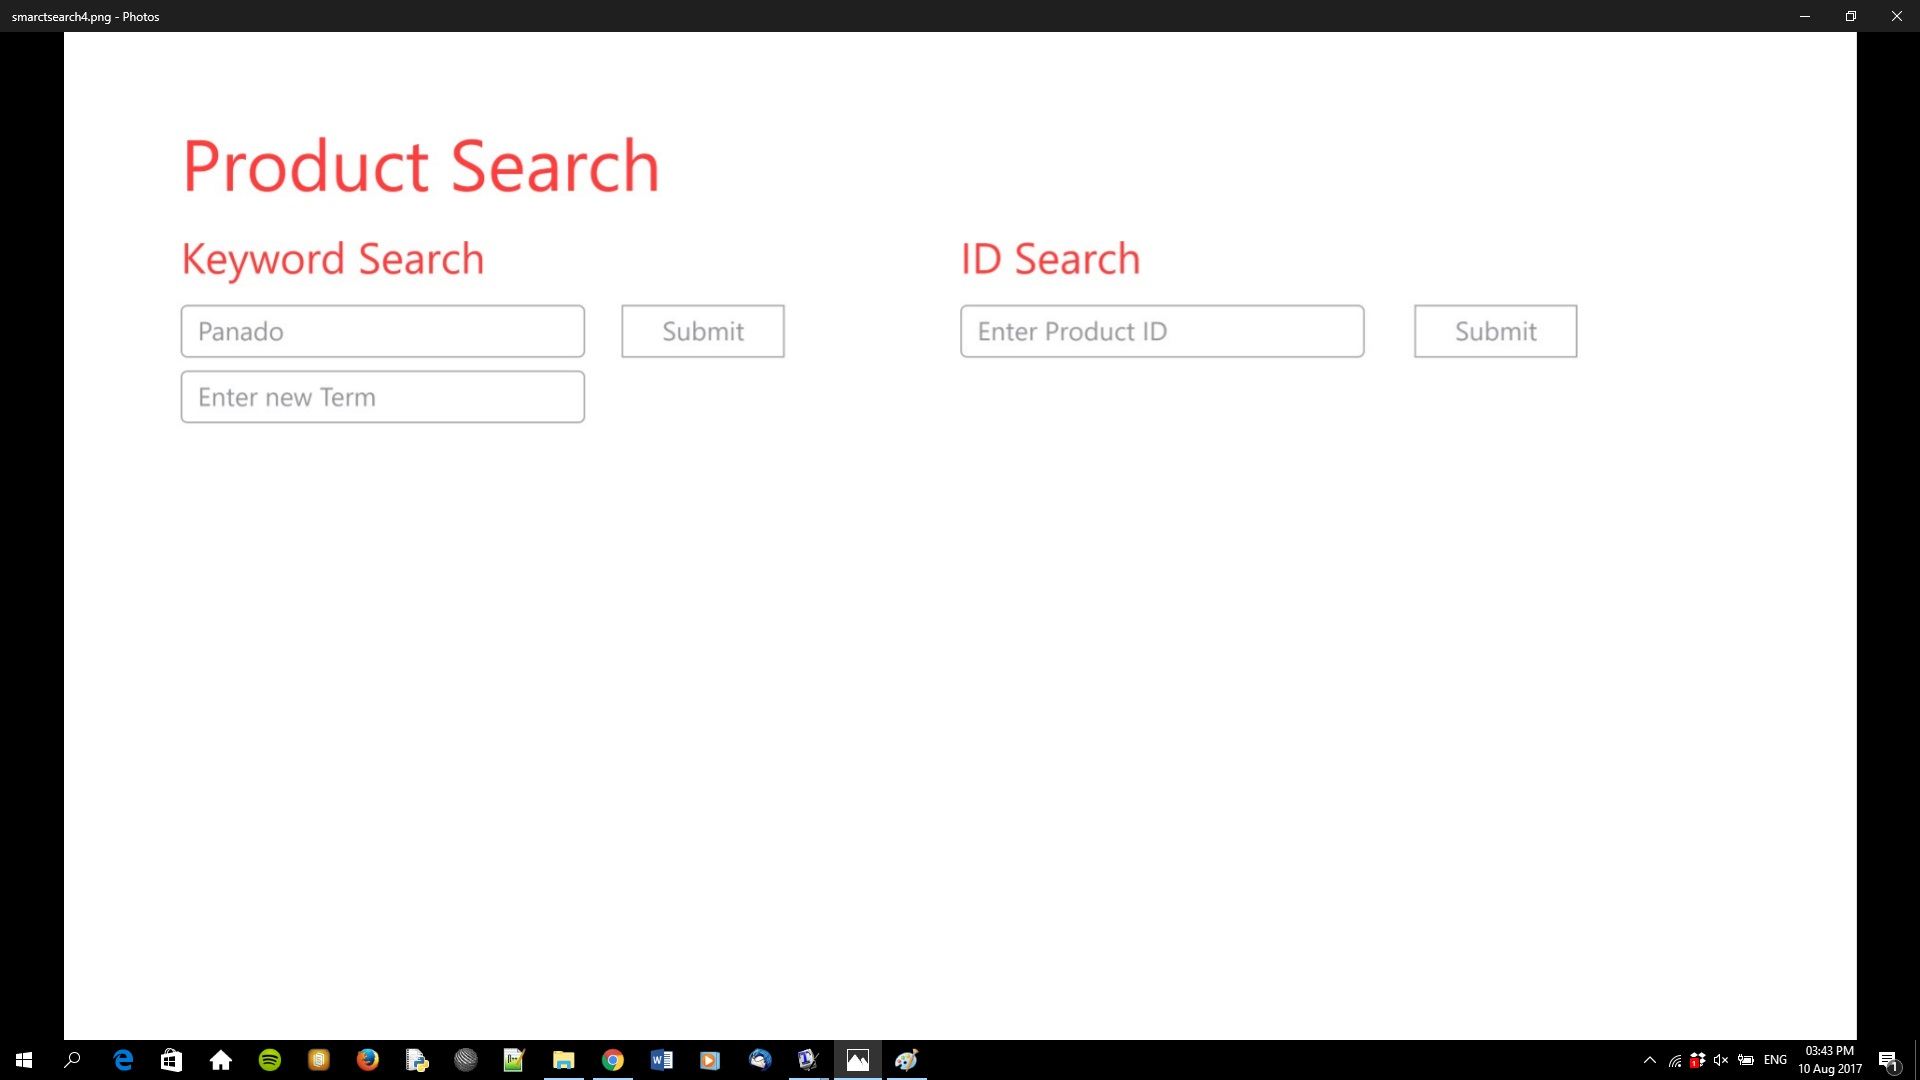
\includegraphics[width=15cm, scale=0.5]{smarctsearch4.jpg}} \\ \\
	{\centering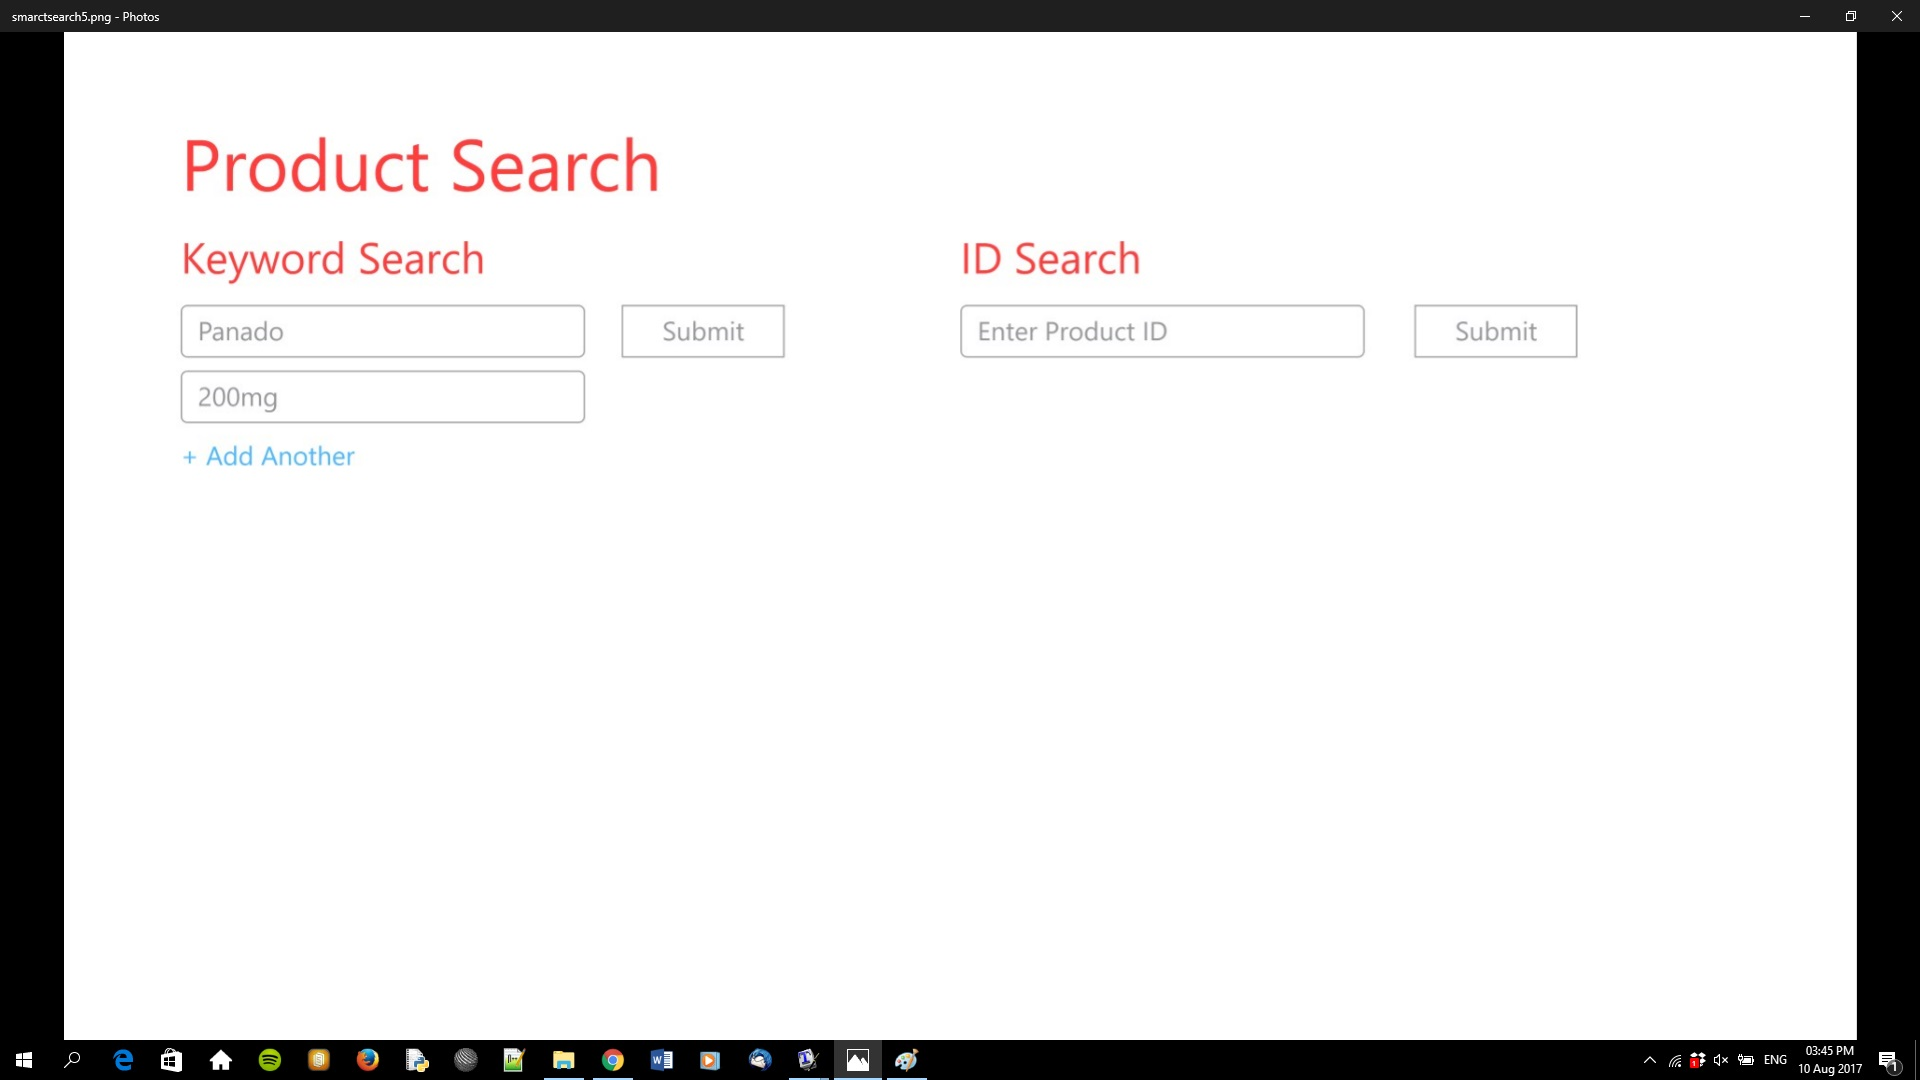
\includegraphics[width=15cm, scale=0.5]{smarctsearch5.jpg}} \\
	\subsection{Search result}
	The result of a search would yield a result below: \\
	{\centering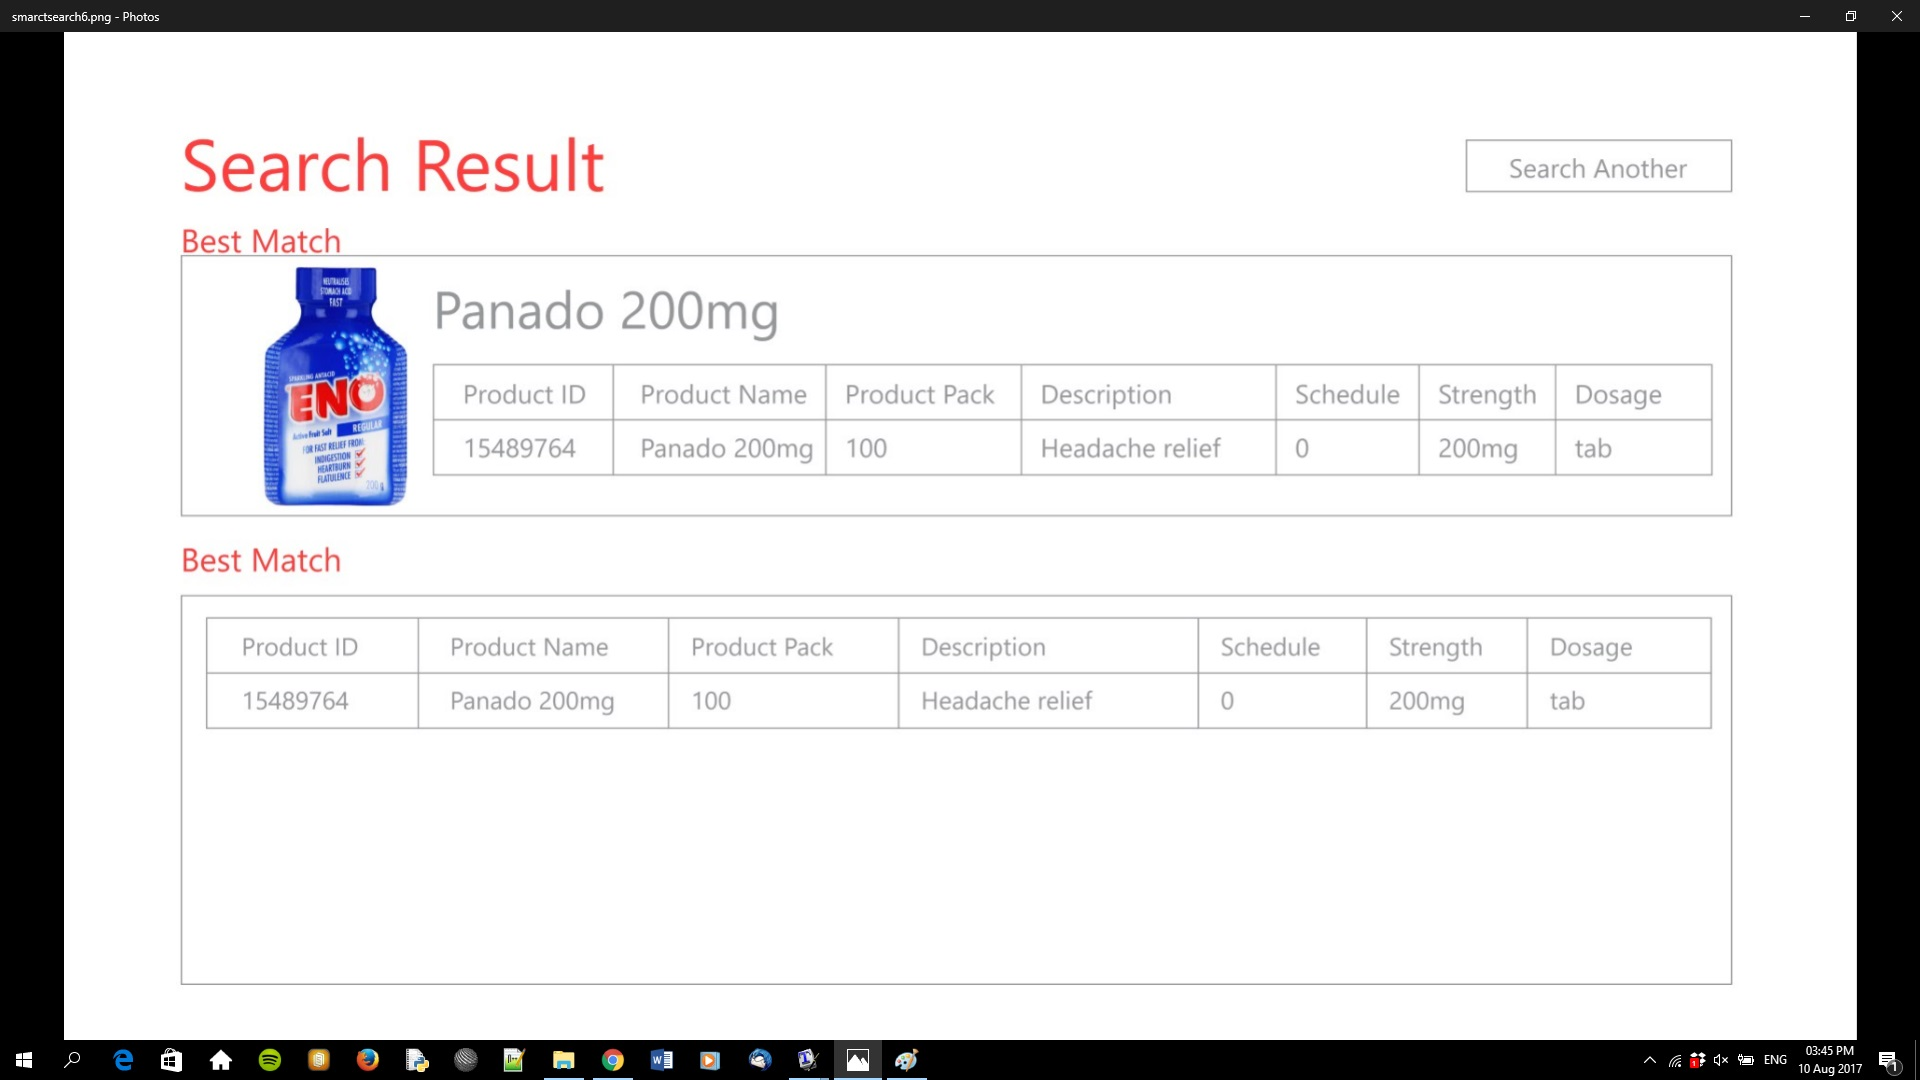
\includegraphics[width=15cm, scale=0.5]{smarctsearch6.jpg}} \\
	
\section{Using the system}
	After registering yourself as a user, you can use the following actions to use the system:
	\begin{enumerate}
	\item Logging In:
		After running the program, you will be presented with a login screen.  In this screen, you will need to provide your username and password to gain access to your account. 
	\item Search:
		After logging in, you will be presented with a screen with an option to search a product by name or by ID. If you would like to search by name, type the name or something close to it, and press search the search button. If you search by ID you need to type the exact ID and then press search.  After pressing search, you will be presented with possible matches to your search.  From here you can select products you are interested to order.
	\item Place Order:
		Not implemented yet. 
	\item Logout:
		After placing an order and have no more to do, remember to logout. To do so, simply press the logout button.

\section{Troubleshooting}



\end{document}
